\subsection{Redes neuronales artificiales}

\paragraph{}Una red neuronal artificial es un algoritmo o clasificador de aprendizaje automático, utilizada tanto para problemas de clasificación como de regresión.
Su concepción está inspirada en parte por la observación de los mecanismos de aprendizaje en sistemas biológicos. Las redes neuronales artificiales están formadas por unidades más simples e interconectadas, donde cada unidad tiene entradas reales y produce una única salida también real, mediante asignación de pesos en regresiones lineales.
Los perceptrones son las unidades sobre las cuales están construidos los sistemas de redes neuronales, dado que por sí solos únicamente puede expresar decisiones lineales, pero su composición en redes neuronales multicapa puede expresar una variedad de funciones objetivo no lineales. 
Un perceptrón recibe valores de $n$ entradas $x_1, x_2, \dots x_n$, realiza una combinación lineal con ellas obteniendo una expresión $x_1 w_1 + x_2 w_2 + \dots x_n w_n$ donde $w_i$ es el peso otorgado a $x_i$, para todo $i \in \{1, \dots, n\}$. Esta expresión es evaluada con una función conocida como \textit{función de activación}, que devuelve un valor de acuerdo a si se supera un umbral determinado o no con la combinación lineal de los valores de entrada. Por ejemplo, si se utiliza a la función signo como función de activación, si la combinación lineal de los valores de entrada supera a un umbral de activación definido por el perceptrón, se devolverá $1$ como salida y $-1$ en caso contrario. La figura \ref{fig:perceptron} muestra la estructura de dicho perceptrón.

\textsc{\begin{figure}[ht!]
	\centering
    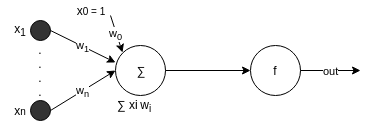
\includegraphics[width=.5\linewidth]{imagenes/perceptron.png}
	\caption{Perceptron con función de activación \textit{f = signo(x)}}
	\label{fig:perceptron}
\end{figure}}

\paragraph{}Cuando se calcula la combinación lineal de los valores de entrada, su valor resultante puede oscilar entre $-\infty$ y $+\infty$, dado que desde un perceptrón no se posee una referencia de cuáles son los límites presentes en las posibles clases de clasificación para el problema de interés. Con el propósito de limitar este valor para producir la salida de un perceptrón es que se usan las funciones de activación. Las funciones de activación utilizadas en este proyecto se detallan a continuación.
La función tanh, expresada de la siguiente manera: $f(x) = tanh(x) = \frac{2}{1 + e^{-2x}} - 1 $ es una función continua no lineal y al componerla consigo misma se obtienen funciones no lineales, lo que permite combinar a unidades o perceptrones con esta función de activación sin perder esa no linealidad. Es una función suave en su curva, mostrando que pequeñas variaciones en valores del dominio cercanos a 0 generan cambios grandes en los valores correspondientes del codominio; esto implica que se le da una gran ponderación a los valores de los extremos del codominio, algo análogo a una tasa de aprendizaje.
La función relu, expresada de la siguiente manera: $f(x) = relu(x) = max(0, x)$ es no lineal y las composiciones de ella consigo misma serán no lineales, pero por su forma, puede generar que algunas neuronas den como resultado cero, constituyéndose una eventual pérdida de información.
Este problema se llama \textit{dying relu problem}. Así también, computar relu es menos costoso que computar tanh porque implica operaciones matemáticas más simples.
La función identity, también llamada de activación lineal, expresada de la siguiente manera: $f(x) = identity(x) = x$, siempre retorna el mismo valor que recibe en su argumento, lo que implica que equivale a una regresión lineal utilizando los pesos de la unidad.

% Backpropagation
\paragraph{}En relación al entrenamiento de las redes neuronales, en este proyecto de grado se utiliza el algoritmo Backpropagation para ajustar los pesos que cada perceptrón de la red asocia a cada una de sus entradas. Dado un nuevo ejemplo de entrenamiento, se generan las salidas que correspondan de la red neuronal, se comparan con las salidas esperadas y si el error es mayor al deseado, se realiza una pasada "hacia atrás" por todos los perceptrones para ajustar sus pesos y se intenta clasificar al ejemplo de entrenamiento nuevamente. Esto se da repetidamente para cada ejemplo de entrenamiento hasta obtener un error aceptable en comparación con la salida esperada de la red neuronal.

% Ventajas y desventajas
\paragraph{}Entre las ventajas de utilizar redes neuronales se encuentran el hecho de que se adecuan correctamente a problemas en los cuales los datos de entrenamiento contienen ruido y en contextos en los cuales tiempos largos de entrenamiento son aceptables. Además, suelen mantener tiempos bajos en clasificación.
Además, como se menciona en la sección \ref{section-trabajos-tecnicas-clasificacion}, una desventaja de las redes neuronales es que su representación interna es difícil de entender para los humanos y por este motivo se dice que se comportan como una “caja negra”.